\documentclass[10pt, onecolumn]{article}
\usepackage{amsmath}
\usepackage{enumerate}
\usepackage{enumitem}
\usepackage{listings}
\usepackage[utf8]{inputenc}
\usepackage{amssymb}
\usepackage{tabularx}
\usepackage{graphicx}

\usepackage{booktabs}
\usepackage{multirow}
\usepackage{siunitx}
\lstset{
    frame=single,
    breaklines=true
}
\usepackage{hyperref}
%\usepackage{atbegshi}
%\AtBeginDocument{\AtBeginShipoutNext{\AtBeginShipoutDiscard}}
%\newcommand{\solution}{\noindent \textbf{Solution:}}
%\documentclass[twoside]{article}
\usepackage[a4paper,outer=1.5cm,inner=1.5cm,top=1.75cm,bottom=1.5cm]{geometry}
\def\mytitle{\textbf{Time Series Autocorrelation}}
\def\myauthor{DUDEKULA USENI}
\def\contact{r171099@rguktrkv.ac.in}
\def\myauthor{DUDEKULA USENI - AHILAN R}
\def\contact{r171099@rguktrkv.ac.in - ra1atcuk@gmail.com}
\def\mymodule{Future Wireless Communication (FWC)}

%\thiswatermark{\centering \put(-15,-100.0){\includegraphics[scale=0.4]{iith.png}} }
\title{\mytitle}
\author{\myauthor\hspace{1em}\\\contact\\FWC22098-FWC22090 -\hspace{0.5em}IITH\hspace{0.5em}\mymodule\hspace{6em}}

\begin{document}
\maketitle
\begin{enumerate}
\section{Abstract}
\item[\textbf{}] Time series autocorrelation

We would like to experiment and see can Raspberry Pi and/or Jetson Nano do time series autocorrelation for large data sets. Data set usually will contain about 40e6 to 1.5e8 points and will be sampled uniformly

\section{Methods used}
Given measurements, $Y_1, Y_2, ..., Y_N$ at time $X_1, X_2, ..., X_N$, the lag $k$ autocorrelation function is defined as
		\[ r_k = \cfrac{\sum_{i=1}^{N-k}(Y_i-\bar{Y})(Y_{i+k}-\bar{Y})}{\sum_{i=1}^N(Y_i-\bar{Y})^2} \]
\subsection{Python only implementation}
This is a Python-only method without any external dependencies for calculating the autocorrelation.
\subsection{Statsmodels}
Statsmodels is a great library for statistics and it provides a simple interface for computing the autocorrelation.
\subsection{numpy correlate}
Numpy provides a simple function for calculating correlation. Since autocorrelation is basically correlation for a data set with itself, we will use numpy.correlate to calculate autocorrelation.
\subsection{Fourier Transform Implementation}
It turns out that autocorrelation is the real part of the inverse Fourier transform of the power spectrum. This follows from the Wiener–Khinchin theorem. We can exploit this, and write the following simple algorithm
\begin{enumerate}
\item Take the Fourier transform of our data set.
\item Calculate the corresponding power spectrum.  
\item Take the inverse Fourier transform of the power spectrum and you get the autocorrelation.
\end{enumerate}
\subsection{Verification of Results}
All the methods produced the same outputs. The output plots are given in the python notebook "acf-codes.ipynb". These results are verified with the standard definition of autocorrelation as convolution of same signal, provide in the verification "verification.ipynb". 
		The output plots are given in the next page.

		\begin{figure}[h!]
\centering
\begin{minipage}{.5\textwidth}
  \centering
  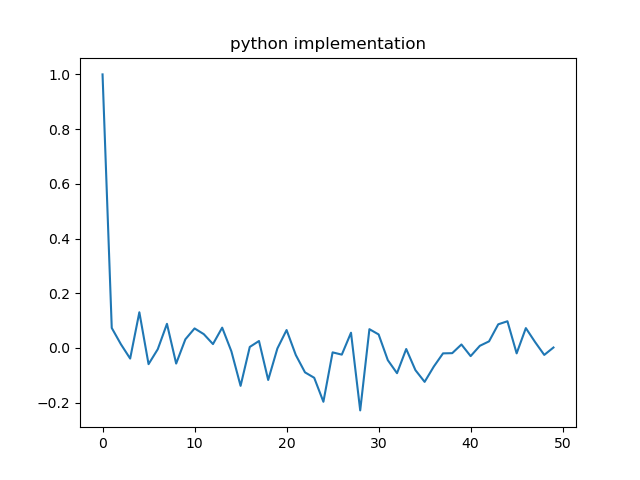
\includegraphics[scale=0.5]{figs/python_imp.png}
	\caption{}
	%\captionof{figure}{A figure}
\label{fig:python_imp}
\end{minipage}%
\begin{minipage}{.5\textwidth}
  \centering
  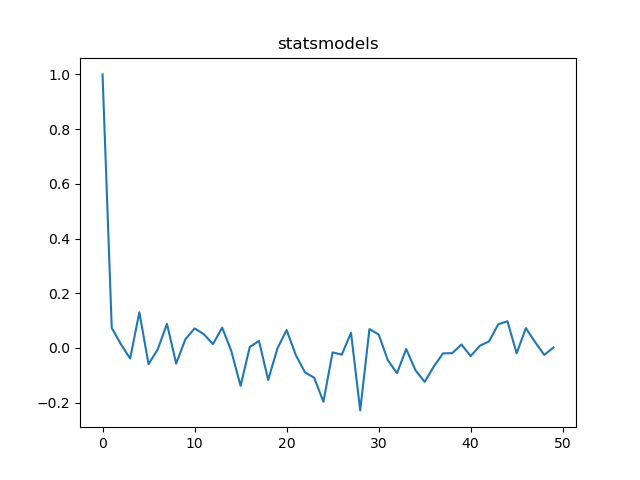
\includegraphics[scale=0.5]{figs/statsmodels.png}
	\caption{}
  %\captionof{}{Another figure}
  %\label{fig:statsmodels}
\end{minipage}
\end{figure}

		\begin{figure}[h!]
\centering
\begin{minipage}{.5\textwidth}
  \centering
  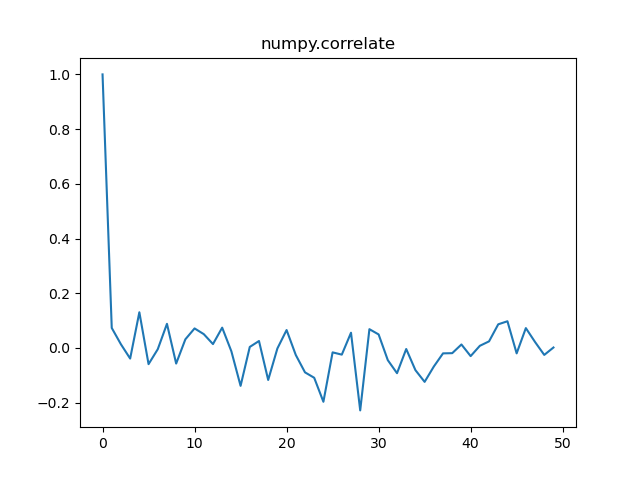
\includegraphics[scale=0.5]{figs/numpy_correlate.png}
	\caption{}
	%\captionof{figure}{A figure}
  \label{fig:numpy_correlate}
\end{minipage}%
\begin{minipage}{.5\textwidth}
  \centering
  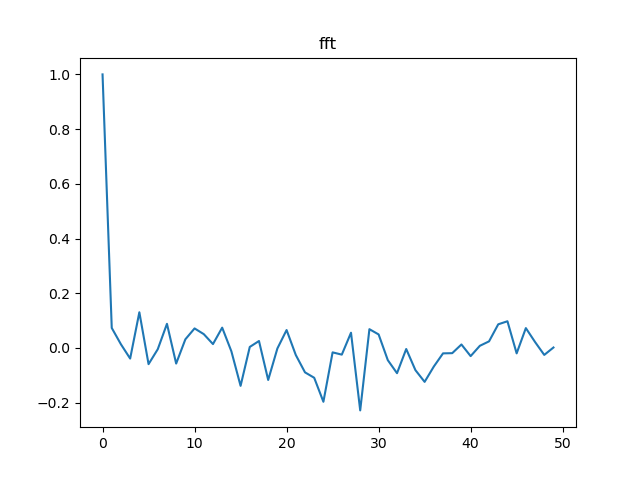
\includegraphics[scale=0.5]{figs/fourier.png}
	\caption{}
  %\captionof{}{Another figure}
  \label{fig:fft}
\end{minipage}
\end{figure}

	\begin{figure}[h!]
\centering
		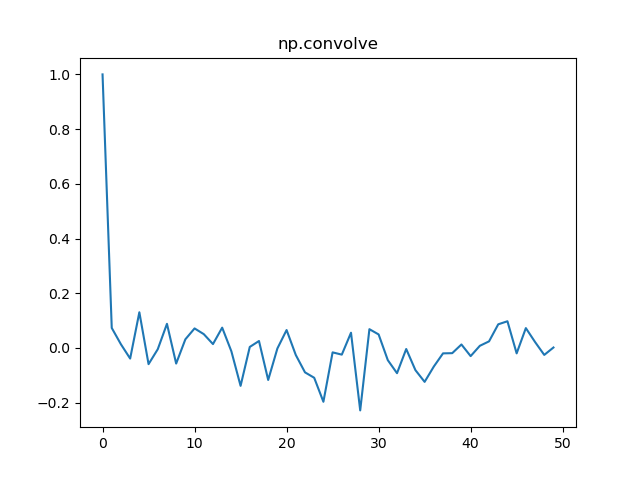
\includegraphics[scale=0.5]{figs/np_convolve.png}
  \caption{Autocorrelation through convolution}
  \label{fig:numpy_convolve}
\end{figure}

		\vspace{5cm}
\section{Perfomance Comparision Tables Of PI And JETSON}

\begin{tabularx}{0.9\textwidth} { 
  | >{\raggedright\arraybackslash}X 
  | >{\centering\arraybackslash}X 
  | >{\centering\arraybackslash}X
  | >{\raggedleft\arraybackslash}X | }
\hline
\multicolumn{3}{|c|}{\textbf{METHOD-1 PYTHON IMPLEMENTATION}} \\
\hline
\textbf{SAMPLES} & \textbf{PI} & \textbf{JETSON}\\
\hline
50K &   36  minutes  & 9 minutes \\ 
\hline
100K &  2.69 hrs     & 52.67 minutes \\  
\hline
200K &  limit time exceed         & limit time exceed \\  
\hline
\end{tabularx}\\


\begin{tabularx}{0.9\textwidth} { 
  | >{\raggedright\arraybackslash}X 
  | >{\centering\arraybackslash}X 
  | >{\centering\arraybackslash}X
  | >{\raggedleft\arraybackslash}X | }
\hline
\multicolumn{3}{|c|}{\textbf{METHOD-2 STATSMODEL}} \\
\hline
\textbf{SAMPLES} & \textbf{PI} & \textbf{JETSON}\\
\hline
50K  &   1.58 sec  & 9.69 sec \\ 
\hline
100K &  2.06 sec   & 28.90 sec \\  
\hline
200K &  2.29 sec   & 1.88 minutes \\  
\hline
%500K &  5    &    13.91 minutes      \\
%\hline
1M  &  3.57 sec &  51.58 minutes            \\     
\hline
10M &  26.03 sec &  limit time exceed           \\
\hline
20M &   Killed  &  killed      \\
\hline
\end{tabularx}\\


\begin{tabularx}{0.9\textwidth} { 
  | >{\raggedright\arraybackslash}X 
  | >{\centering\arraybackslash}X 
  | >{\centering\arraybackslash}X
  | >{\raggedleft\arraybackslash}X | }
\hline
\multicolumn{3}{|c|}{\textbf{METHOD-3 NUMPY.CORRELATE}} \\
\hline
\textbf{SAMPLES} & \textbf{PI} & \textbf{JETSON}\\
\hline
50K  &   4.701 sec  & 6.80 sec \\ 
\hline
100K &  11.37 sec   & 27.18 sec \\  
\hline
200K &  1.89 minutes   & 1.89 minutes \\  
\hline
%500K &      &  13.96 minutes       \\
%\hline
1M  &  1.90 minutes & 52.96 minutes             \\     
\hline
10M &  limit time exceed & limit time exceed             \\
\hline
20M &   Killed  &  killed      \\
\hline
\end{tabularx}\\


\begin{tabularx}{0.9\textwidth} { 
  | >{\raggedright\arraybackslash}X 
  | >{\centering\arraybackslash}X 
  | >{\centering\arraybackslash}X
  | >{\raggedleft\arraybackslash}X | }
\hline
\multicolumn{3}{|c|}{\textbf{METHOD-4 FOURIER TRANSFORM}} \\
\hline
\textbf{SAMPLES} & \textbf{PI} & \textbf{JETSON}\\
\hline
50K  &   0.08 sec  & 1.49 sec \\ 
\hline
	100K &  0.16 sec   & 2.70 sec \\  
\hline
	200K &  0.39 sec   & 5.27 sec \\  
\hline
%	500K &      &      12.49 sec  \\
%\hline
	1M  &  0.51 sec &    24.98 sec          \\     
\hline
	10M &  44.20 sec &    52.19 sec         \\
\hline
	20M &   Killed  &  killed      \\
\hline
\end{tabularx}\\
\section{Conclusion}
Overall, RaspberryPi is faster to execute the autocorrelation than Jetson Nano. However, both have limitaions depending on the number of samples taken and the method of implementation. For example, when 20 million samples were taken both output produced "killed".
\section{Software}
 Download the following code
 \begin{lstlisting}
https://github.com/ahilan22/fwc/tree/main/jetson-pi
 \end{lstlisting}
%https://github.com/dudekulauseni123/FWC0982022

\end{enumerate}
\end{document}
%\end{document}
